\section{validity confirmation through Union Bound}
\label{sec4}
 In this section, in order to confirm the validity of our proposed method, we obtain a union bound using the low-weight codewords with weight-$2$ and weight-$3$ PC or SC and compare it with that obtained via the transfer function as well as simulation results.

\subsection{A novel union bound}
Let $\bbA_h(d)$ be the set of all $a(x)$ which yields weight-$d$ PCs \ie, $w_H(h(x))=w_H(a(x)f(x))=d$. Similarly, we also define $\bbA_b(d)$ and $\bbA_c(d)$ as the sets of all $a(x)$s which result in weight-$d$ SCs and codewords, respectively.

Then, for $w_H(b(x)), w_H(h(x)) \geq 2$, we have from \eqref{eq:cw-weight} that
\begin{align}
\bbA_c(d) = \bigcup_{\ell = 2}^{d-2} \left\{\bbA_b(\ell) \cap \bbA_h(d-\ell)\right\}
\label{Eq:exactset}
\end{align}
Now, we replace the set $\bbA_c(d)$ by the following approximated set %\eqref{setApprox}
\begin{equation}
\begin{split}
\bbA_c(d) \approx \bbA_c'(d) &= \left\{\bigcup_{\ell = 2}^{\ell+1} \left\{\bbA_b(\ell) \cap \bbA_h(d-\ell)\right\}\right\}\\
&\bigcup \left\{\bigcup_{\ell = 2}^{\ell+1} \left\{\bbA_b(d-\ell) \cap \bbA_h(\ell)\right\}\right\}\\
\end{split}
\label{setApprox}
\end{equation}
and obtain an approximated union bound as
\begin{align}
P_b \leq \frac{1}{k} \sum_{d=d_{\text{free}}}^{d_{\text{free}+1}} \sum_{a(x) \in \cA'_c(d)}w_H(a(x)g(x)) Q\Bigg( \sqrt{\frac{2dE_c}{N_0}}\Bigg)
\label{novelEq7}
\end{align}
Notice that since $\bbA_c(d)$ in \eqref{Eq:exactset} is replaced by $\bbA_c'(d)$, the contributions of the codewords with $\ell \approx d-\ell$ may be neglected in our approximation.

To obtain $\bbA_c'(d)$, based on $f(x)$, we first generate the set consisting of $a(x)$s which yield the weight-2 and -3 PCs, \ie~$\bbA_h(2)\cup\bbA_h(3)$. Next, for each $a(x) \in \bbA_h(2)\cup\bbA_h(3)$, we determine the corresponding SC $b(x)=a(x)g(x)$. Similarly, we determine the PC $h(x)=a(x)f(x)$ for each $a(x)$ in the set $\bbA_b(2)\cup\bbA_b(3)$  obtained based on $g(x)$. Finally, we narrow down the corresponding codewords as $w_H(b(x))+w_H(h(x)) \leq d_{\text{free+1}}$ for $a(x) \in \bbA_h(2)\cup\bbA_h(3)\cup\bbA_b(2)\cup\bbA_b(3)$.

As examples, in Table \ref{code-tables-1},\ref{code-tables-2} and \ref{code-tables-3}, we listed the low-weight PCs and SCs found by our proposed method for the codes listed in Table \ref{TB:Codes} with the corresponding example numbers where each polynomial appeared in.
\begin{table}[htbp]
	\caption{The generator polynomials}
	\centering
	\begin{tabular}{cll} 
		\toprule
			& $f(x)$ & $g(x)$ \\ %[0.5ex] 
		\midrule
		Code I & $1+x^2$ & $1+x+x^2$\\
		(5/7) &  (Ex. \ref{Ex:4}) &  (Ex. \ref{Ex:1}) \\\hline
		Code I& $1+x+x^2+x^3+x^4$& $1+x^4$\\
		(37/21) &  (Ex. \ref{Ex:3}) &  (Ex. \ref{Ex:4})\\\hline
		Code III& $1+x+x^4$& $1+x^2+x^3+x^4$\\
		(23/35) &  (Ex. \ref{Ex:2}) &  (Ex. \ref{Ex:5})\\
		\bottomrule
	\end{tabular}
	\label{TB:Codes}
\end{table}

\subsection{Numerical results}
We obtained the approximated union bound by \eqref{novelEq7} for the codes listed in Table \ref{TB:Codes}  and compared them with that obtained using the transfer function in Figures \ref{simFig1}-\ref{simFig3}.
For reference purpose, the details of the PCs and SCs used for drawing the bound are listed in Tables \ref{code-tables-1} - \ref{code-tables-3} with the extra codewords found by computer search (labelled as `Not Found').

In these figures, we also evaluated BER through computer simulations. To plot BER points, we assume each RSC code is BPSK modulated and transmitted over the AWGN channel with a frame with size of $N=64$. At the receiver, the Viterbi algorithm is used to recover the transmitted bits and we accumulated more than 1,000 bits errors for obtain each plot point.

\begin{table}[hbp]
		\caption{SCs and PCs for Code I}
		\centering
		\begin{tabularx}{0.48\textwidth}{|c|c|XXX} 
			\toprule
			$w_H(c(x))$& ~ & $a(x)$ & $b(x)$ & $h(x)$ \\ %[0.5ex] 
			\midrule
			5&Found&$1$ & $1+x+x^{2}$ & $1+x^2$\\
			\cline{1-5}
			6&~&$1+x$ & $1+x^3$ & $1+x+x^2+x^3$\\
			&Found&$1+x^2$ & $1+x+x^3+x^4$ & $1+x^{4}$\\
			&~&$1+x+x^2$ & $1+x^2+x^4$ & $1+x+x^3+x^4$\\
			&~&$1+x+x^3$ & $1+x^4+x^5$ & $1+x+x^2+x^5$\\
			\bottomrule
		\end{tabularx}		
		\label{code-tables-1}
	\end{table}
	
\begin{table}[htbp]
		\caption{SCs and PCs for Code II}
		\centering
		\begin{tabularx}{0.48\textwidth}{|c|c|XXX} 
			\toprule
			$w_H(c(x))$&~& $a(x)$ & $b(x)$ & $h(x)$ \\ %[0.5ex] 
			\midrule
			6&Found&$1+x$ & $1+x+x^{4}+x^5$ & $1+x^5$\\
			\cline{1-5}
			7&Found&$1$ & $1+x^4$ & $1+x+x^2+x^3+x^4$\\
			\bottomrule
		\end{tabularx}		
		\label{code-tables-2}
	\end{table}

	
\begin{figure}[hbp]
	\centering
	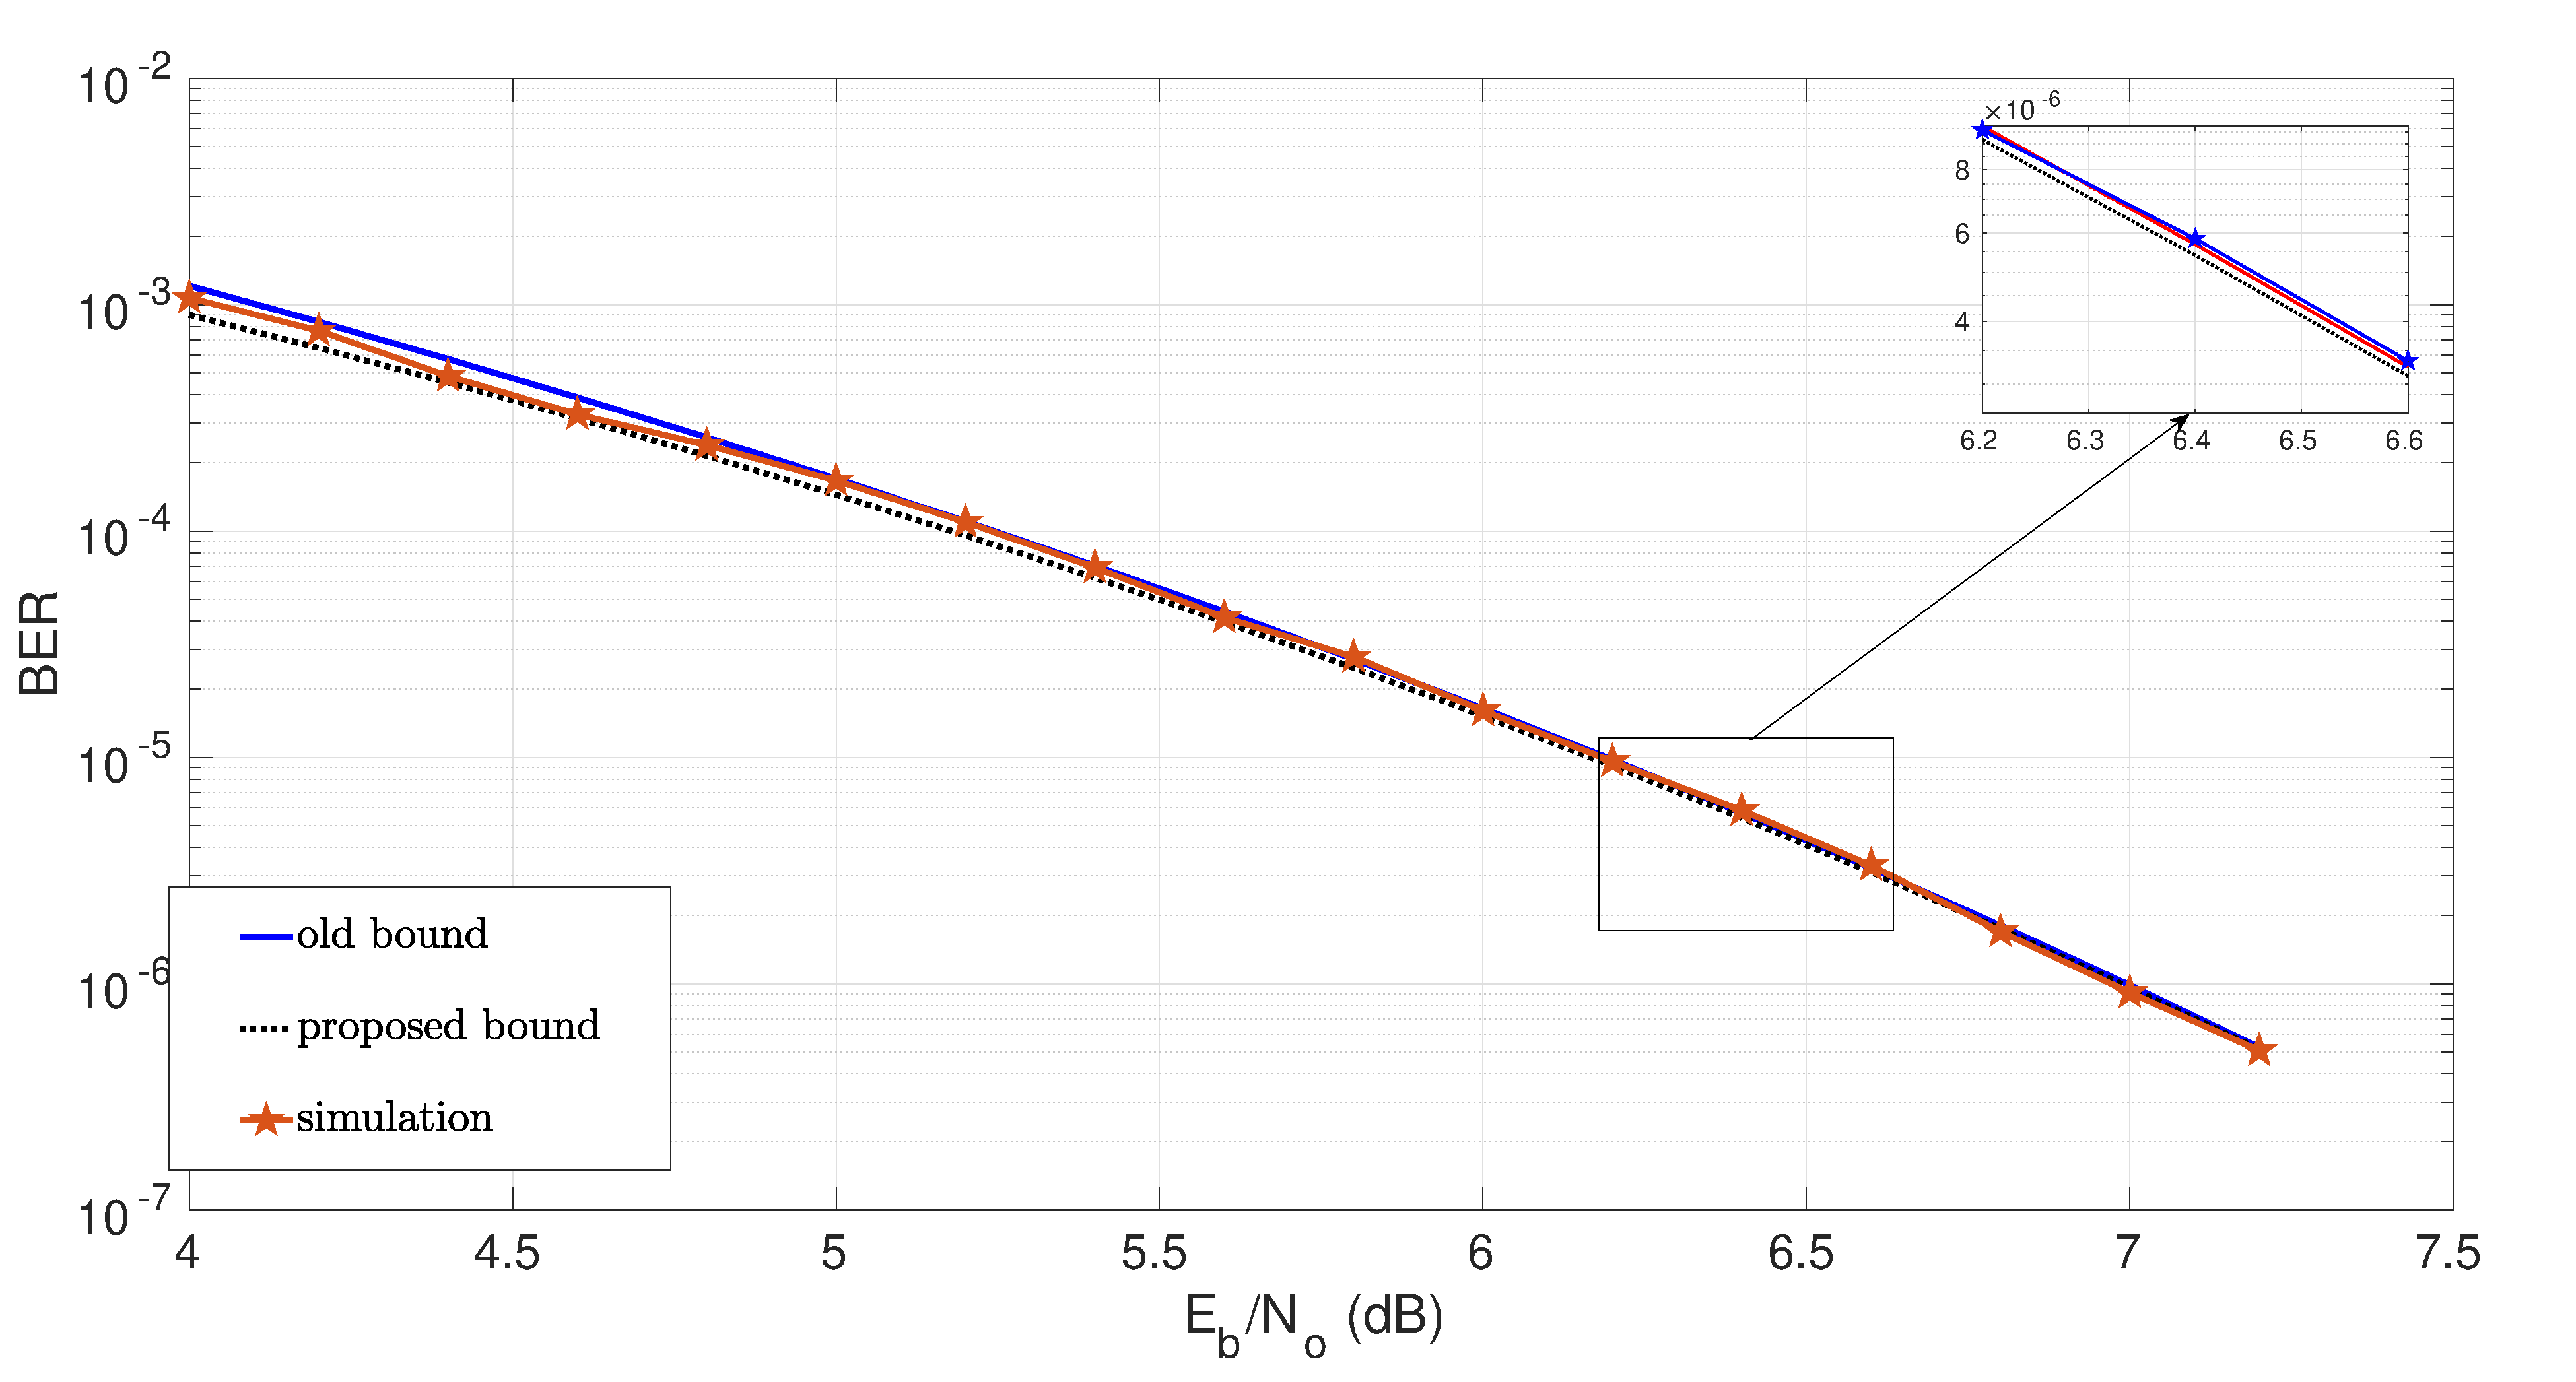
\includegraphics[width=0.48\textwidth]{./Images/RSC_5_7_lower_weights4.eps}
	\captionof{figure}{Old Bound vs New Bound vs Simulation for 5/7 RSC Code}
	\label{simFig1}
\end{figure}

As shown in Table \ref{code-tables-1}, since the free distance of the 5/7 RSC code is 5, the codewords consisting of weights 2 and 3 SCs or PCs are taken into account in the proposed method,thus all codewords with weights up to 6 are picked up. Also, Fig. \ref{simFig1} indicates that the union bound obtained using the codewords with weights up to $d_{\rm free+1}$ tracks the BER curve with sufficient accuracy, especially in the high $E_b/N_0$ region. Moreover, the bounds obtained by our method and the transfer function converge to the same value with $E_b/N_0$ increament and match the simulation results well.  

For the 37/21 RSC code, since the free distance of the code is 6, there is no counting omission in the proposed method for codewords with weight up to 7 and the BER curve can be well approximated using the codewords with weight 6 and 7 with a high accuracy at the high $E_b/N_0$ region.

\begin{figure}[htbp]
	\centering
	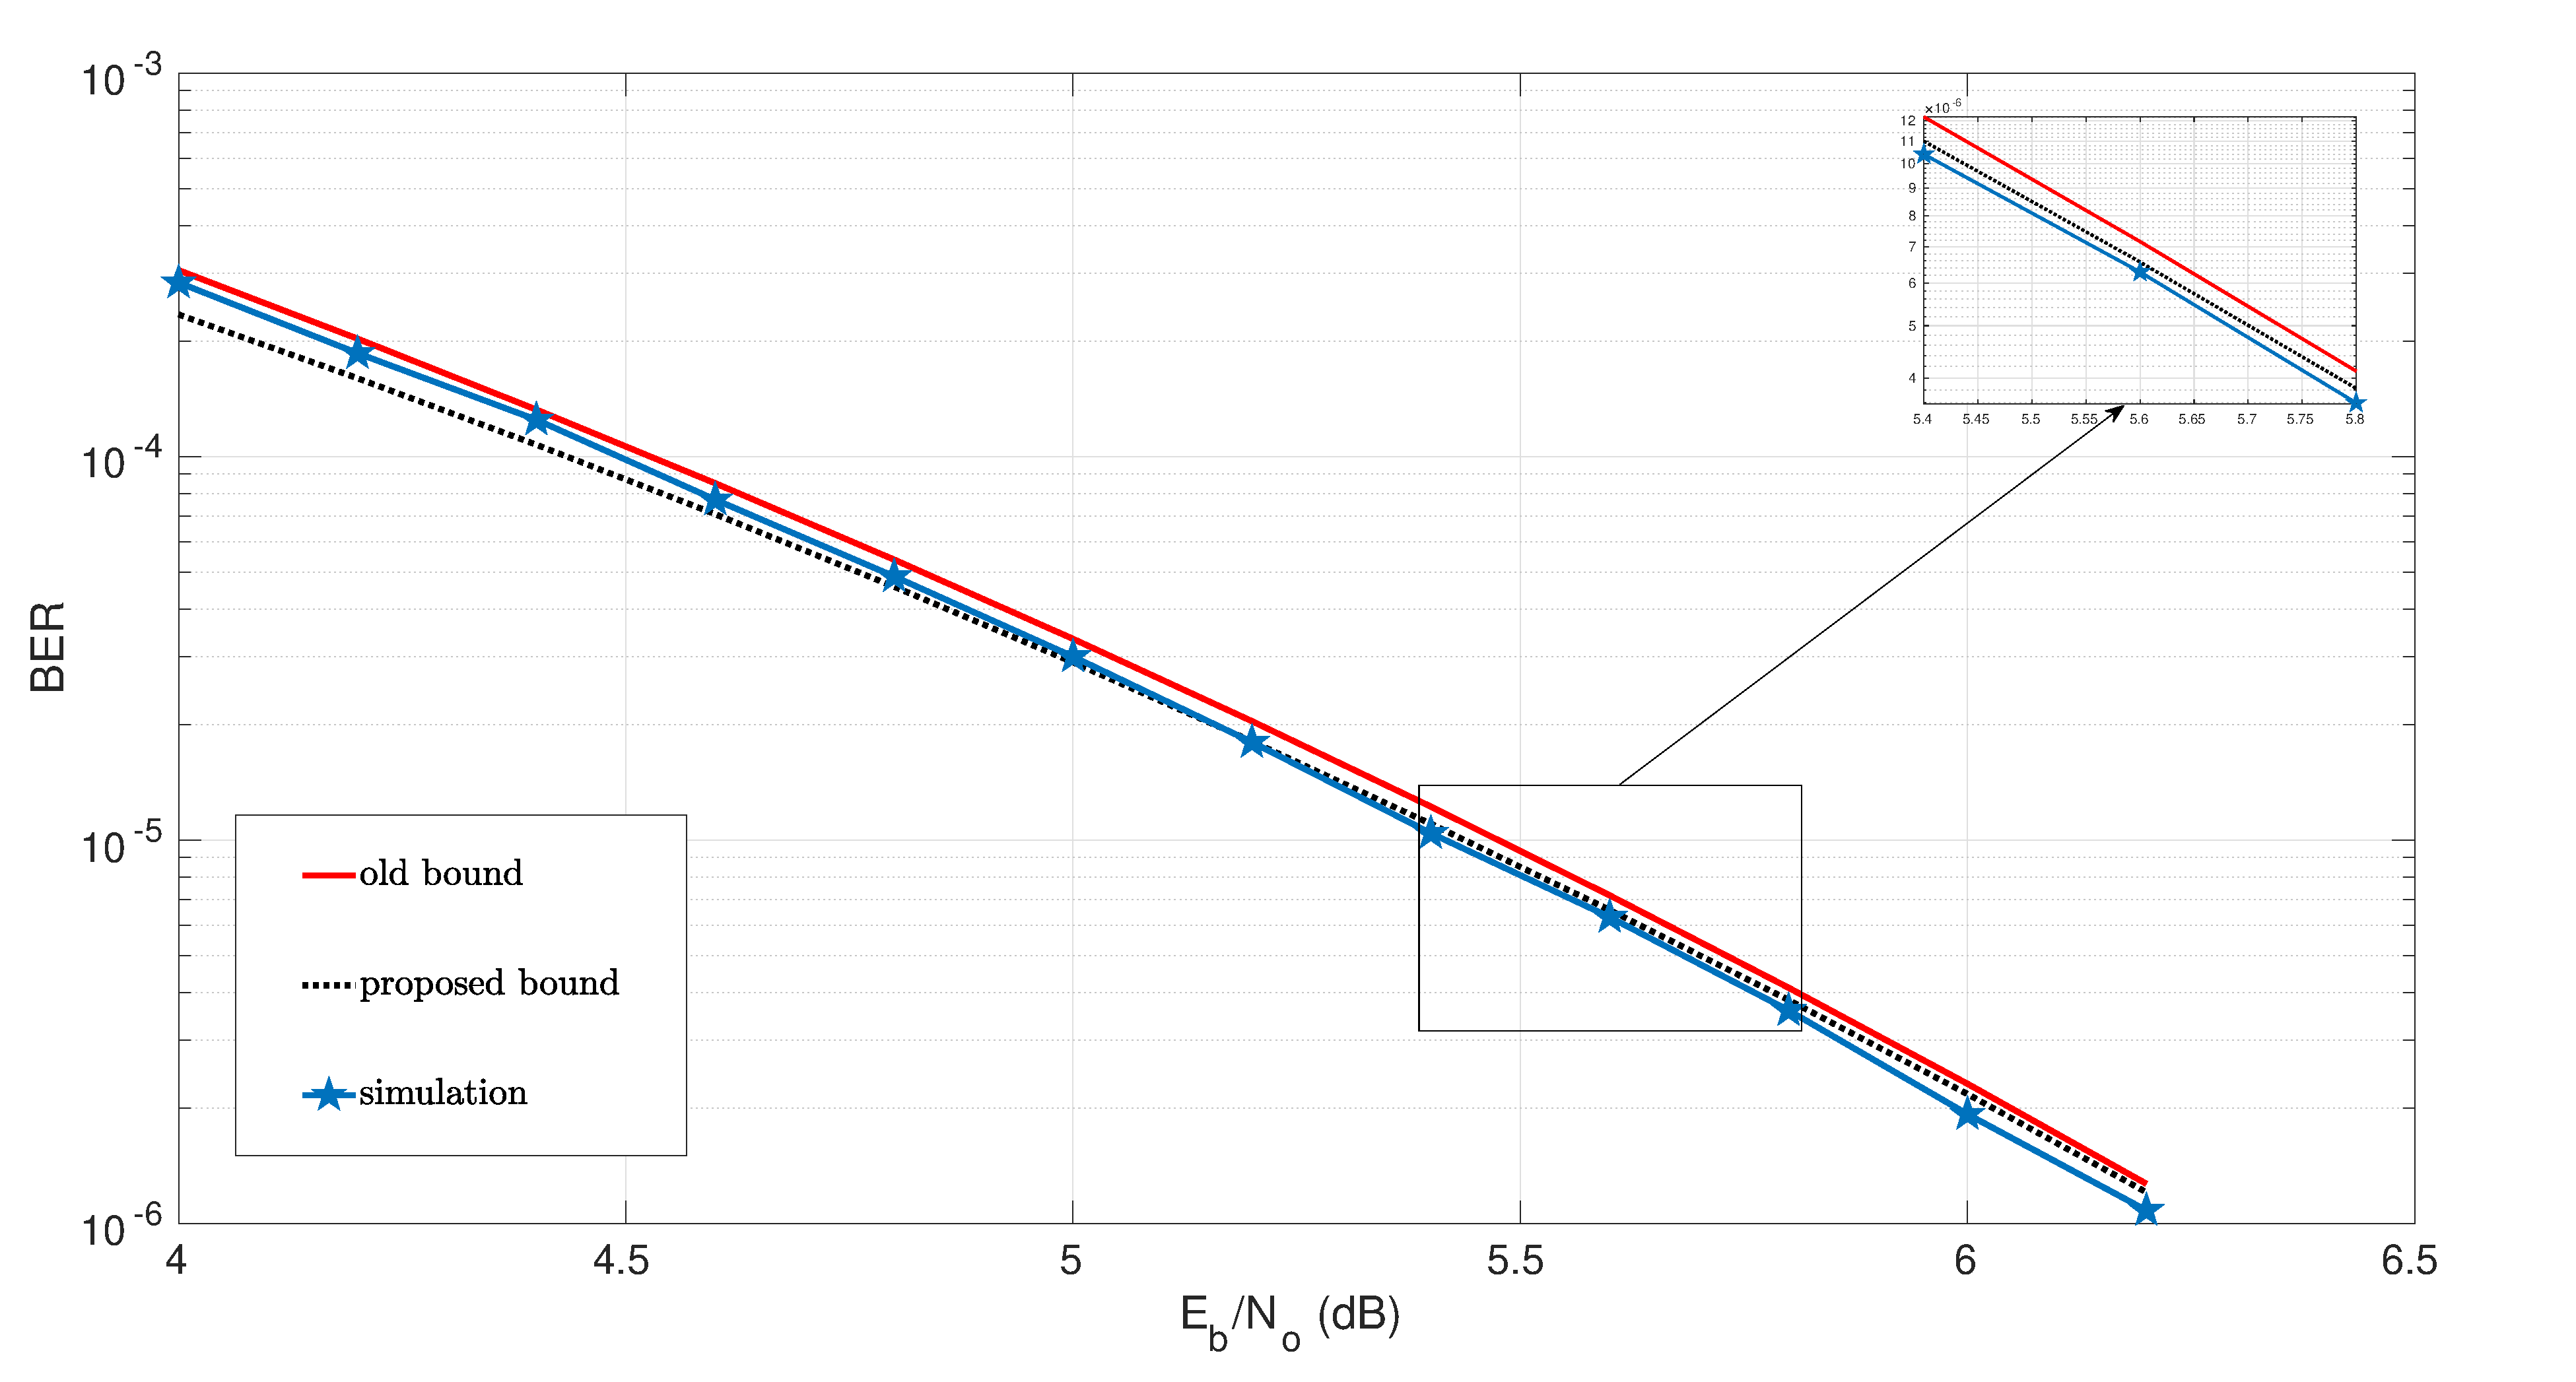
\includegraphics[width=0.48\textwidth]{./Images/RSC_37_21_lower_weights4.eps}
	\caption{Old Bound vs New Bound vs Simulation for 37/21 RSC Code}
	\label{simFig2}
\end{figure}

For the code III, the free distance is 7 and the proposed method identifies 2 codewords with weight-7 while 3 codewords with weight-8 can not be found as shown in Table \ref{code-tables-3}. Thus, while we use the weight-7 codewords to approximate the BER curve as Fig. \ref{simFig3}, there about a 0.1 dB gap between the proposed method and simulation results.

\begin{figure}[htbp]
	\centering
	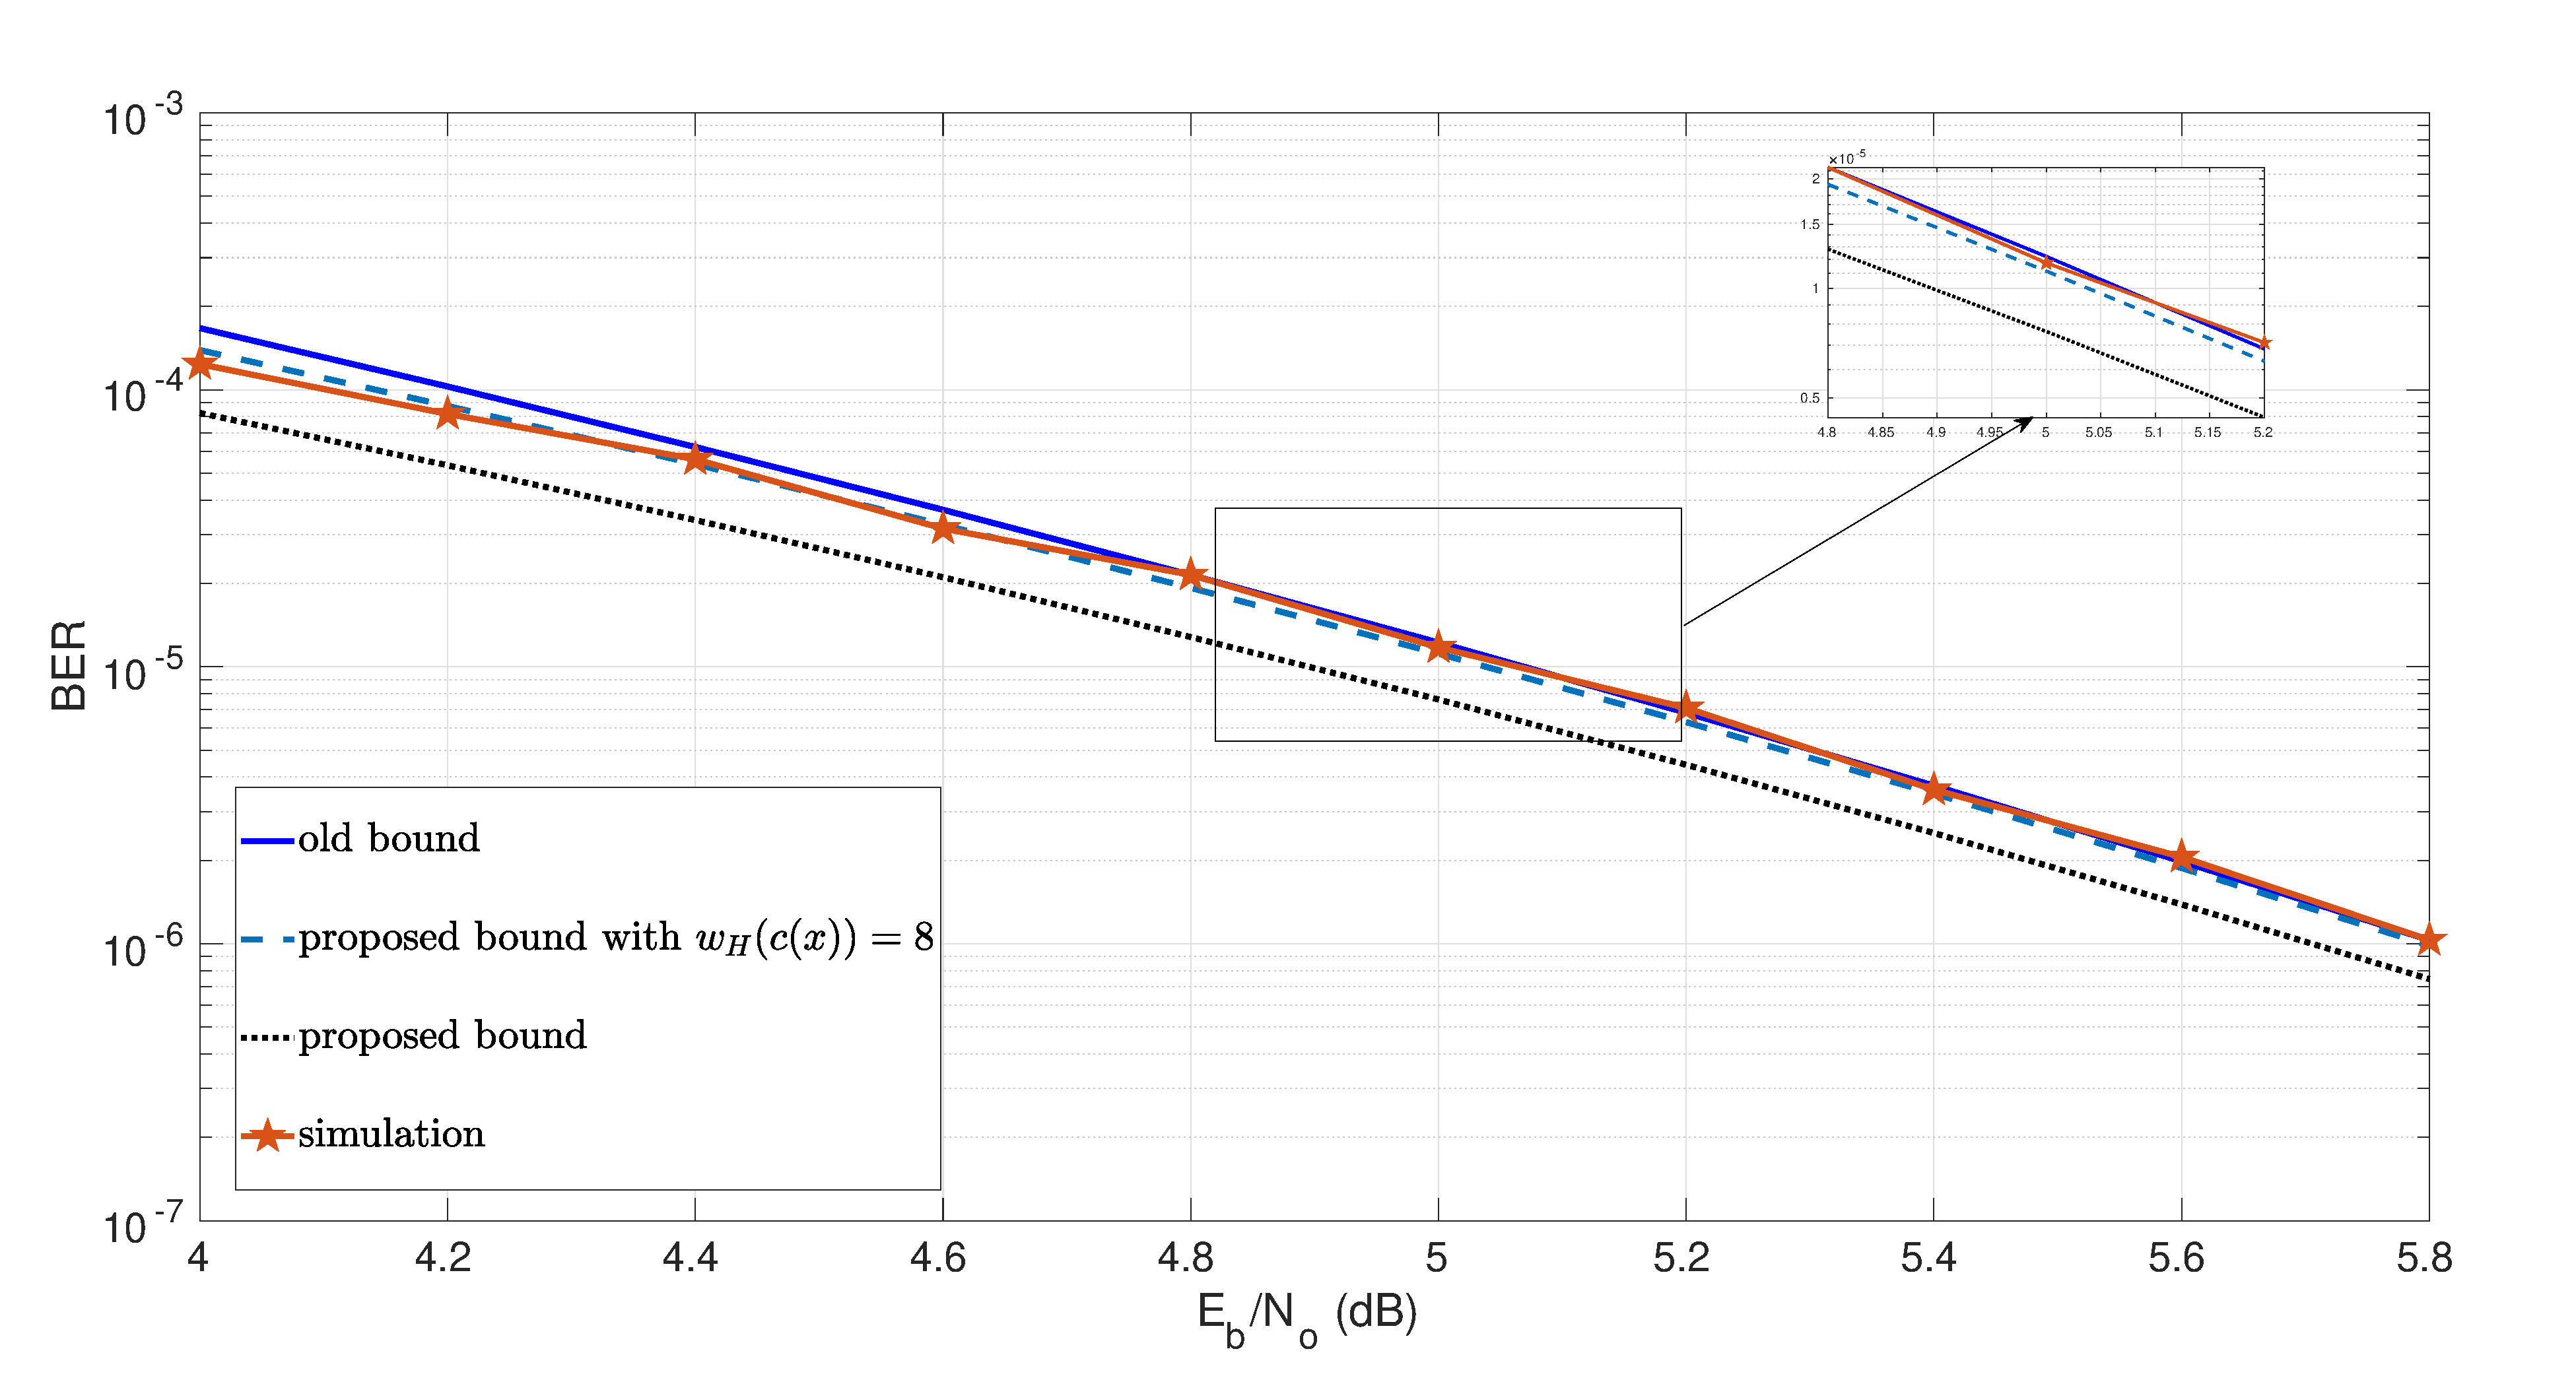
\includegraphics[width=0.48\textwidth]{./Images/RSC_23_35_lower_weights4.eps}
	\caption{Old Bound vs New Bound vs Simulation for 23/35 RSC Code}
	\label{simFig3}
\end{figure}

\begin{table}[htbp]
		\caption{SCs and PCs for Code III}
		\centering
		\begin{tabularx}{0.48\textwidth}{|c|c|XXX} 
			\toprule
			$w_H(c(x))$&~& $a(x)$ & $b(x)$ & $h(x)$ \\ %[0.5ex] 
			\midrule
			7&Found&$1$ & $1+x^2+x^3+x^4$ & $1+x+x^{4}$\\
			  &~&$1+x^2+x^3$ & $1+x^7$ & $1+x+x^2+x^6+x^7$\\
			\cline{1-5}
			&&$1+x$ 						& $1+x+x^2+x^5$ 			& $1+x^2+x^4+x^5$\\
			8&Not Found&$1+x+x^2+x^4$ 				& $1+x+x^7+x^8$ 			& $1+x^3+x^6+x^8$\\
			&&$1+x+x^2+x^4+x^6+x^7$ 	& $1+x+x^6+x^{11}$ 			& $1+x^3+x^{10}+x^{11}$\\
			\bottomrule
		\end{tabularx}		
		\label{code-tables-3}
	\end{table}





